\documentclass{article}





\usepackage{fullpage}
\usepackage{nopageno}
\usepackage{amsmath}
\usepackage{amsfonts}
\usepackage{graphicx}
\usepackage{framed}
\usepackage{algorithmic}
\usepackage{xcolor}

\definecolor{dark_red}{rgb}{0.5,0.0,0.0}
\definecolor{dark_green}{rgb}{0.0,0.5,0.0}
\definecolor{dark_blue}{rgb}{0.0,0.0,0.5}
\definecolor{blue}{rgb}{0.0,0.0,1.0}

\newcommand{\dr}[1]{\textcolor{dark_red}{#1}}
\newcommand{\dg}[1]{\textcolor{dark_green}{#1}}
\newcommand{\db}[1]{\textcolor{dark_blue}{#1}}
\newcommand{\blue}[1]{\textcolor{blue}{#1}}



\title{PS2 Host}


\begin{document}



\section*{debouncer}

The {\bf debouncer} filters short transient pulses from a signal, ensuring that there are no accidental transitions that may result in unwanted behavior. 

\begin{center}
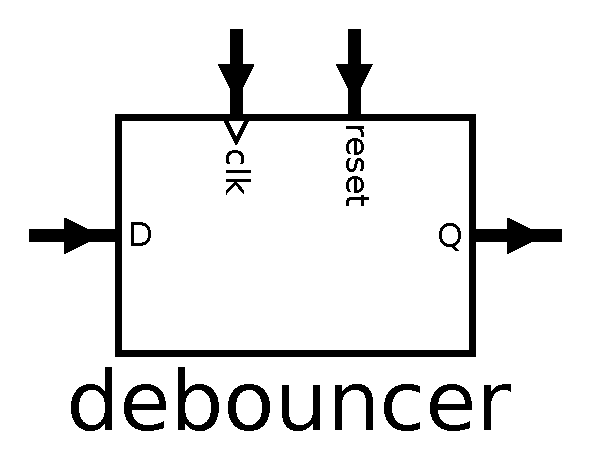
\includegraphics[width = 0.6\textwidth]{debouncer}
\end{center}

{\bf Port descriptions:} 
\begin{itemize} 
\item Input port \texttt{clk} a clock with a 10ns period
\item Input port \texttt{reset} an asynchronous reset port.  
\item Input port \texttt{D} is the debouncer input. 
\item Output port \texttt{Q} is the debouncer output.
\end{itemize}

{\bf The internal signals are:} 
\begin{itemize}
\item Multi-bit signal \texttt{counter} counts down to the time where the input has been stable for long enough to merit a transit a change in the output. The number of bits in this counter can be customized through the use of a generic field. 
\item Signal \texttt{i\_D} buffers the input port \texttt{D}. 
\item Signal \texttt{i\_Q} buffers the output port \texttt{Q}.
\end{itemize}

\vspace{2mm}

{\bf Behavioral description:}

\vspace{5mm}

When \texttt{reset} is high, the input \texttt{D} writes straight through to the output. 

The value of \texttt{i\_D} lags that of \texttt{D} by 1 clock cycle, so \texttt{D} and \texttt{i\_D} can be used to detect changes in the input \texttt{D}. 

When a change has been detected, \texttt{counter} is reset to its maximum value. This maximum value can be customized through the use of a generic field.   

When a change is not detected, if the counter is \(0\), then the input writes through to the output, otherwise the counter decreases by 1.  



\section*{ps2\_host}

\begin{center}
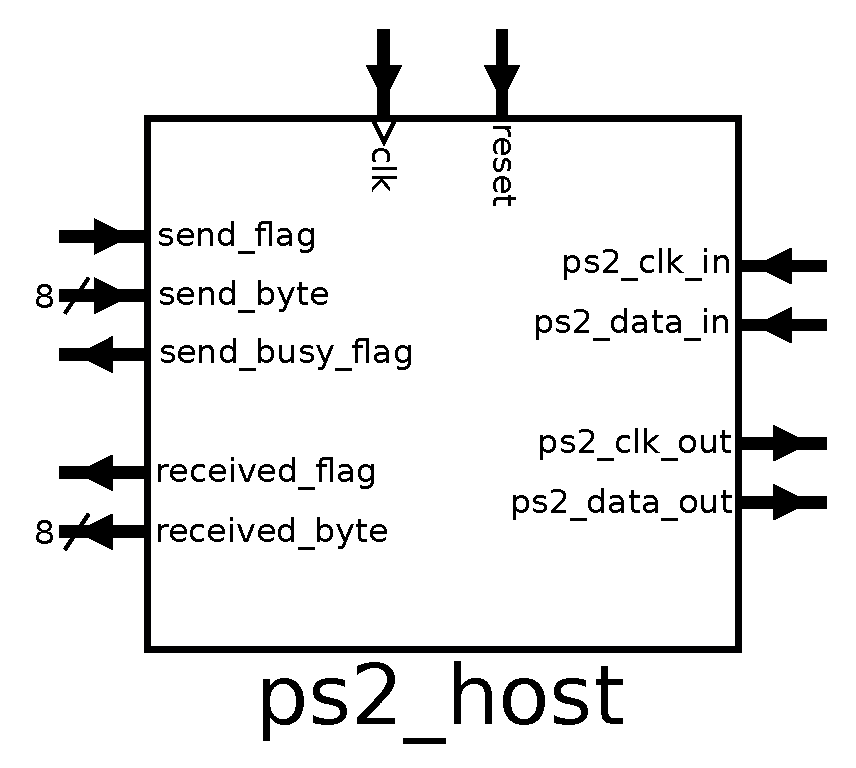
\includegraphics[width = \textwidth]{ps2_host}
\end{center}

{\bf Port descriptions:}
\begin{itemize}
\item Input port \texttt{clk} a clock with a 10ns period
\item Input port \texttt{reset} an asynchronous reset port.  
\item Input port \texttt{ps2\_clk\_in} is the input ps2 clock connection. {\bf This port connects to a remote device.} 
\item Input port \texttt{ps2\_data\_in} is the input ps2 data connection. {\bf This port connects to a remote device.} 
\item Output port \texttt{ps2\_clk\_out} is the output ps2 clock connection. {\bf This port connects to a remote device.} 
\item Output port \texttt{ps2\_data\_out} is the output ps2 data connection. {\bf This port connects to a remote device.} 
\item Output \(8\)-bit port \texttt{received\_byte} returns bytes that the host receives from the ps2 connection. 
\item Output port \texttt{received\_flag} is a flag that is normally \texttt{0}, but emits a {\bf 1 clock period} pulse on the clock cycle where \texttt{received\_byte} is returning the byte received from the ps2 connection. 
\item Input \(8\)-bit port \texttt{send\_byte} is the byte that is to be sent over the ps2 connection. 
\item Input port \texttt{send\_flag} is given a {\bf 1 clock period} pulse on the clock cycle where \texttt{send\_byte} is set to the byte that is to be sent over the ps2 connection. 
\item Output port \texttt{send\_busy\_flag} is \texttt{1} when an existing byte is queued to be sent or is being sent, and no new bytes are currently being accepted.         
\end{itemize}

{\bf The internal signals are:}
\begin{itemize}
\item Signal \texttt{i\_ps2\_clk} is the input \texttt{ps2\_clk\_in} signal filtered through a debouncer to eliminate transient pulses less than 1\(\mu\)s in duration. 
\item Signal \texttt{i\_ps2\_data} is the input \texttt{ps2\_data\_in} signal filtered through a debouncer to eliminate transient pulses less than 1\(\mu\)s in duration. 
\item Signal \texttt{i\_ps2\_clk\_d1} is \texttt{i\_ps2\_clk} delayed by 1 clock cycle to detect falling edges in \texttt{i\_ps2\_clk}. 
\item Signal \texttt{i\_ps2\_clk\_falling\_edge} is high when the current value of \texttt{i\_ps2\_clk} is 0, while the value on the previous clock cycle is 1. 
\item Signal \texttt{i\_direction} has 3 states: \texttt{S\_DIR\_IDLE}, \texttt{S\_DIR\_RECEIVE}, \texttt{S\_DIR\_SEND}. These states denote the following: 
	\begin{itemize}
	\item \texttt{S\_DIR\_IDLE} denotes the state where no data is begin received or transmitted.  
	\item \texttt{S\_DIR\_RECEIVE} denotes the state where a byte is being received. 
	\item \texttt{S\_DIR\_SEND} denotes the state where a byte is being sent. Note that a single byte can be primed for sending even if the state is currently \texttt{S\_DIR\_RECEIVE}. When the state returns to \texttt{S\_DIR\_IDLE}, it will then be set to \texttt{S\_DIR\_SEND} and transmission will begin immediately.    
	\end{itemize} 
%%%%%%%%%%%%%%
\item Signal \texttt{i\_data\_received\_state} has 6 states: \texttt{S\_REC\_IDLE}, \texttt{S\_REC\_BITS}, \texttt{S\_REC\_PARITY}, \texttt{S\_REC\_STOP}, \texttt{S\_REC\_DONE}, \texttt{S\_REC\_ERROR}. These states denote the following: 
	\begin{itemize}
	\item \texttt{S\_REC\_IDLE} denotes the state where no byte is being received. This is the state when \texttt{i\_direction} is not \texttt{S\_DIR\_RECEIVE}. When \texttt{i\_direction} is \texttt{S\_DIR\_IDLE}, and a falling ps2 clock edge has been detected, this signals a transition of \texttt{i\_data\_received\_state} to either \texttt{S\_REC\_BITS} or \texttt{S\_REC\_ERROR} depending on the ps2 data line (a valid start bit should always be 0).
	\item \texttt{S\_REC\_BITS} denotes the state where data bits are expected to be sent over the ps2 data line. A new bit is read with each falling ps2 clock edge, and is registered. When a total of 8 bits have been received in this state, sate \texttt{S\_REC\_PARITY} begins. 
	\item \texttt{S\_REC\_PARITY} denotes the state where the parity bit is now expected. When this bit arrives, the next state is either \texttt{S\_REC\_STOP} or \texttt{S\_REC\_ERROR} depending on the status of the parity bit.  
	\item \texttt{S\_REC\_STOP} denotes the state where the stop bit is now expected. When this bit arrives, the next state is either \texttt{S\_REC\_DONE} or \texttt{S\_REC\_ERROR} depending on whether of not the stop bit is correctly 1 or not.
	\item \texttt{S\_REC\_DONE} denotes a successful receipt of a byte from the remote device. {\bf This state lasts for exactly 1 clock cycle}, after which the next state is \texttt{S\_REC\_IDLE}.   
	\item \texttt{S\_REC\_ERROR} denotes a failed receipt of a byte from the remote device. {\bf This state lasts for exactly 1 clock cycle.}, after which the next state is \texttt{S\_REC\_IDLE}. 
	\end{itemize}   
\item \(8\)-bit signal \texttt{i\_received\_data\_buffer} stores the bits received from the ps2 data line. 
\item \(3\)-bit signal \texttt{i\_received\_data\_bit\_index} stores an index from \(0\) to \(7\), the index of the bit that is being expected. 
\item Signal \texttt{i\_received\_data\_parity\_bit} stores the current parity as the bits are received. 
\item \(17\)-bit signal \texttt{i\_receive\_time\_out\_counter} is a counter that counts the clock ticks since the last falling ps2 clock edge. If 1ms passes without a falling ps2 clock edge, it will be assumed that there was an error in transmission, and the receipt is aborted, turning \texttt{i\_data\_received\_state} to \texttt{S\_REC\_ERROR}, eventually returning \texttt{i\_direction} to \texttt{S\_DIR\_IDLE}. 
%%%%%%%%%%%%%%
\item Signal \texttt{i\_send\_busy\_flag} is an internal register for the \texttt{send\_busy\_flag} output port. 
\item Signal \texttt{i\_data\_send\_state} has 9 states: \texttt{S\_SEND\_IDLE}, \texttt{S\_SEND\_INHIBIT}, \texttt{S\_SEND\_BITS}, \texttt{S\_SEND\_PARITY}, \texttt{S\_SEND\_STOP}, \texttt{S\_SEND\_PS2\_RELEASE}, \texttt{S\_SEND\_ACKNOWLEDGE}, \texttt{S\_SEND\_DONE}, \texttt{S\_SEND\_ERROR}. These states denote the following: 
	\begin{itemize}
	\item \texttt{S\_SEND\_IDLE} denotes the state where no byte is being currently sent. This is the state when \texttt{i\_direction} is not \texttt{S\_DIR\_SEND}. When \texttt{i\_direction} becomes \texttt{S\_DIR\_SEND}, the state transitions to \texttt{S\_SEND\_INHIBIT}, the ps2 clock is forced low, and a countdown counter (\texttt{i\_send\_inhibitor\_counter}) for the inhibit pulse is set to 150\(\mu\)s.
	\item \texttt{S\_SEND\_INHIBIT} denotes the state where the ps2 clock is being inhibited by being forced to 0. This state lasts until the inhibitor counter, \texttt{i\_send\_inhibitor\_counter}, reaches 0 wherein the ps2 clock is released (set to 1) and the ps2 data port is taken control of and forced low. The next state is \texttt{S\_SEND\_BITS}.   
	\item \texttt{S\_SEND\_BITS} denotes the state where a bit is assigned to the ps2 data port on each falling ps2 clock edge. After the 8 bits comes \texttt{S\_SEND\_PARITY}. 
	\item \texttt{S\_SEND\_PARITY} denotes the state where the parity bit is sent on the falling ps2 clock edge. Next is \texttt{S\_SEND\_STOP}. 
	\item \texttt{S\_SEND\_STOP} denotes the state where the stop bit, namely 1, is sent on the falling ps2 clock edge. Next is \texttt{S\_SEND\_ACKNOWLEDGE}.  
	\item \texttt{S\_SEND\_ACKNOWLEDGE} denotes the state where the ps2 data port is to receive a 0 on the last falling ps2 clock edge. If this 0 is received, the next state is \texttt{S\_SEND\_DONE}, otherwise the next state is \texttt{S\_SEND\_ERROR}. 
	\item \texttt{S\_SEND\_DONE} denotes a successful transmission of a byte to the remote device. {\bf This state lasts for exactly 1 clock cycle}, after which the next state is \texttt{S\_SEND\_IDLE}.   
	\item \texttt{S\_SEND\_ERROR} denotes a failed transmission of a byte to the remote device. {\bf This state lasts for exactly 1 clock cycle.}, after which the next state is \texttt{S\_SEND\_IDLE}. The transmission is immediately re-attempted.
	\end{itemize}
\item \(8\)-bit signal \texttt{i\_send\_data\_buffer} stores the bits that are to be sent to the ps2 data line.   
\item \(3\)-bit signal \texttt{i\_send\_data\_bit\_index} stores an index from \(0\) to \(7\), the index of the bit that is being sent.  
\item Signal \texttt{i\_send\_data\_parity\_bit} stores the current parity as the bits are sent.    
\item \(15\)-bit signal \texttt{i\_send\_inhibitor\_counter} is a counter that counts down to the end of the inhibitor pulse. 
\end{itemize} 

\vspace{2mm}

%{\bf Behavioral description:}

\vspace{5mm} 







\end{document}










